\documentclass[10pt,twocolumn,letterpaper]{article}

\usepackage{cvpr}
\usepackage{times}
\usepackage{epsfig}
\usepackage{graphicx}
\usepackage{amsmath}
\usepackage{amssymb}

\usepackage{url}

% Include other packages here, before hyperref.
\usepackage{algorithm}
\usepackage{algpseudocode}
% If you comment hyperref and then uncomment it, you should delete
% egpaper.aux before re-running latex.  (Or just hit 'q' on the first latex
% run, let it finish, and you should be clear).
%\usepackage[pagebackref=true,breaklinks=true,letterpaper=true,colorlinks,bookmarks=false]{hyperref}

\cvprfinalcopy % *** Uncomment this line for the final submission

\def\httilde{\mbox{\tt\raisebox{-.5ex}{\symbol{126}}}}

% Pages are numbered in submission mode, and unnumbered in camera-ready
\ifcvprfinal\pagestyle{empty}\fi
\begin{document}

\title{Comparison between a sequential and a multithreading version of the mean shift clustering algorithm}

\author{Emilio Cecchini\\
{\tt\small emilio.cecchini@stud.unifi.it}
}


\maketitle
\thispagestyle{empty}


\begin{abstract}
In this paper, after a brief introduction to the mean shift clustering, a sequential version will be compared with a multithreading version of the algorithm. The obtained speedup with a multi-core CPU will be analyzed using a different number of threads. The algorithm is written in C++ and the parallel version is obtained with OpenMP. The focus of this paper and his associated code do not consist in showing a very efficient version of the mean shift clustering algorithm, but rather in analyzing the performance improvements obtainable with a  multithreading version compared to a sequential one.
\end{abstract}

\section{Introduction}

Since there are many variations of the mean shift algorithm, in this section I will describe the specific version used in my implementation.

%-------------------------------------------------------------------------
\subsection{Mean shift}

The mean shift algorithm is a nonparametric clustering technique that does not require as input the number of clusters to look for.  It is based on the concept of \textit{kernel density estimation} or \textit{KDE}, that is a method to estimate the underlying distribution for a set of data.

At each step, a \textit{kernel function} is applied to each point that causes the points to shift in the direction of the local maxima determined by the kernel. The iterations end when all points reach the maxima of the underlying distribution estimated by the chosen kernel.

There are many different types of kernel, the most used is the \textit{Gaussian kernel}:

\begin{align}
k(x) =  e^{-\dfrac{x}{2\sigma^2}}
\end{align}

The standard deviation $\sigma$ is the \textit{bandwidth} parameter. Depending on the kernel bandwidth parameter used, the resultant density function will vary: with a high bandwith value you will get a few large clusters and vice versa.

The new location where to shift each point at each step of the algorithm is computed as a weighted average between the point and its neighbors, where the weights are calculated with the Gaussian kernel. Suppose $x$ is a point to be shifted and $N(x)$ are the sets of points near to that point. Let $dist(x, x_i)$ be the distance from the point $x$ to the point $x_i$. The new position $x'$ where $x$ has to be shifted is computed as follows:

\begin{align}
x' = \dfrac{\sum_{x_i \in N(x)} k(dist(x,x_i)^2) x_i}{\sum_{x_i \in N(x)} k(dist(x, x_i)^2)}
\end{align}

The mean shift algorithm applies that formula to each point iteratively until they converge, that is until the position does not change.

\section{Sequential version}

The algorithm is very simple: each point shifts towards the maxima of its underlying distribution. The algorithm ends when all the points have stopped shifting.

Here is the pseudocode of the core of the algorithm:

\begin{algorithm}
\label{MeanShiftAlgSeq}
\caption{Mean shift core}
\begin{algorithmic}

    \While{allPointsHaveStoppedShifting()}
            \For{each point $p$}
                \If{hasStoppedShifting($p$)}
                    \State \textbf{continue}
                \EndIf
            \State shift($p$)
            \EndFor
    \EndWhile

\end{algorithmic}
\end{algorithm}

To speed up the process, the shifting process of a point is stopped when the distance from its older position is less than an epsilon value specified by the user.

The main data structures used by the algorithm are two lists. The first list contains all the original points in their original positions, the second list is where the new positions are stored after a shifting step. The list containing the original positions remains unchanged during the algorithm; at each step, the new position where to perform the shift is computed by reading the points in this list, so it is important to notice that each point perform its shifting operations completely independently from the other points.

\section{Parallel version}

\subsection{The algorithm}

The mean shift algorithm is a embarrassingly parallel work: each point perform its shifting independently from the other points. This makes it the perfect case for using the OpenMP technology. In fact, with a single \verb"pragma" command it was possible to switch from a sequential version to a parallel version.

Here is the pseudocode of the parallel version of the core algorithm:

\begin{algorithm}
\label{MeanShiftAlgPar}
\caption{Mean shift core parallel}
\begin{algorithmic}

    \While{allPointsHaveStoppedShifting()}
        \State \#pragma omp parallel for schedule(dynamic)
            \For{each point $p$}
                \If{hasStoppedShifting($p$)}
                    \State \textbf{continue}
                \EndIf
            \State shift($p$)
            \EndFor
    \EndWhile

\end{algorithmic}
\end{algorithm}

Note that the only difference from the sequential version in \ref{MeanShiftAlgSeq} is the \verb"pragma" statement. That statement is placed just before the \verb"for" loop, in this way there is no need of any critical sections. If it had been placed before the \verb"while" loop, then the parallel algorithm would have been more complex introducing an overhead due to the synchronization between threads.

\subsection{Data structures}

The data structures used by the parallel algorithm are the same of the sequential version.

There is a list containing the original points that is shared among the threads. This list is never changed during the computation, so there is not need of any synchronization mechanism.

The other list, that one containing the new positions of the shifted points, is shared among the threads too, but also in this case no synchronizations are necessary because the parallelized section is the computation of the shifting and after each shifting step there is an implicit barrier at the end of the \verb"for" loop. At each step, each thread computes the new position of a set of points independently from the others.

\subsection{Thread scheduling}

Not all the points need the same number of steps to reach the final position. In the same dataset some point could converge very quickly while others could perform a larger number of shifting operations. That's why we have to make sure that each thread receives the same amount of workload.

With OpenMP it is possible to change the workload of the \verb"for" loop assigned to each thread. By default, OpenMP uses a \textit{static scheduling}, where the entire \verb"for" loop is divided statically in chunks of equal size. This kind of scheduling is not optimal for this problem, because, as we have noticed before, each point perform a different number of steps depending on how fast it converges to the center of its cluster. So it could be happen that a thread finishes very soon its iterations and then it has to wait the other threads wasting computational resources.

The best scheduling strategy for this algorithm is the \textit{dynamic scheduling}, where the iterations are assigned to the threads while the loop is executing. Assigning the workload to the threads in this way should ensure that each thread will never stop its execution waiting for the others.

To perform a dynamic scheduling we have to write in the \verb"pragma" statement the clause \verb"schedule(dynamic)". With that directive an interation is assigned to a thread as soon as the thread has finished the computation of the previously assigned iteration.

We report a table containing the comparison between the executions of a parallel version with a static scheduling and a dynamic scheduling. The test was performed on a machine with an Intel Xeon CPU 2.00 \textit{GHz} with 8 cores on a data set of $50000$ points of three dimensions:

\begin{table}[H]
\centering
\begin{tabular}{ccc}
\hline
\textbf{Threads} & \textbf{Static} (\textit{seconds}) & \textbf{Dynamic} (\textit{seconds}) \\
\hline
2 & 703.729 & 695.051 \\
3 & 467.874 & 465.511 \\
4 & 351.299 & 345.102 \\
5 & 378.612 & 325.376 \\
6 & 320.762 & 306.645 \\
7 & 300.665 & 289.901 \\
8 & 277.214 & 277.058 \\
\hline
\end{tabular}
\end{table}

We can notice that the dynamic scheduling adoption leads to a faster execution because the workload is better distributed among the threads.

\section{Speedup analysis}

To compare the performance of a sequential algorithm with a parallel version, the main measure used is the \textit{speedup}, that is the ration between the execution time of the sequential version and the execution time of the parallel version with the same input.

\begin{align}
S = \dfrac{t_S}{t_P}
\end{align}

Ideally, the speedup should be the number of processor used to perform the parallel version.

In this case, the speedup is computed with a script that first executes a sequential version, then it executes on the same data set differents parallel versions using a different number of threads. In this section are reported some results obtained with datasets of different sizes.

The tests were performed on a machine with an Intel Xeon CPU 2.00 \textit{GHz} with eight cores.

\begin{table}[H]
\begin{tabular}{c c c}
\hline
\textbf{Number of points} & \multicolumn{2}{l}{100} \\
\hline
\textbf{Sequential time} & \multicolumn{2}{l}{0.0060} \\
\hline
\textbf{Threads} & \textbf{Time} (seconds) & \textbf{Speedup} \\
\hline
2 & 0.0040 & 1.52 \\
3 & 0.0035 & 1.74 \\
4 & 0.0027 & 2.22 \\
5 & 0.0024 & 2.47 \\
6 & 0.0024 & 2.45 \\
7 & 0.0025 & 2.35 \\
8 & 0.0031 & 1.94 \\
9 & 0.0047 & 1.29 \\
10 & 0.0135 & 0.45 \\
\end{tabular}
\end{table}

\begin{figure}[H]
\centering
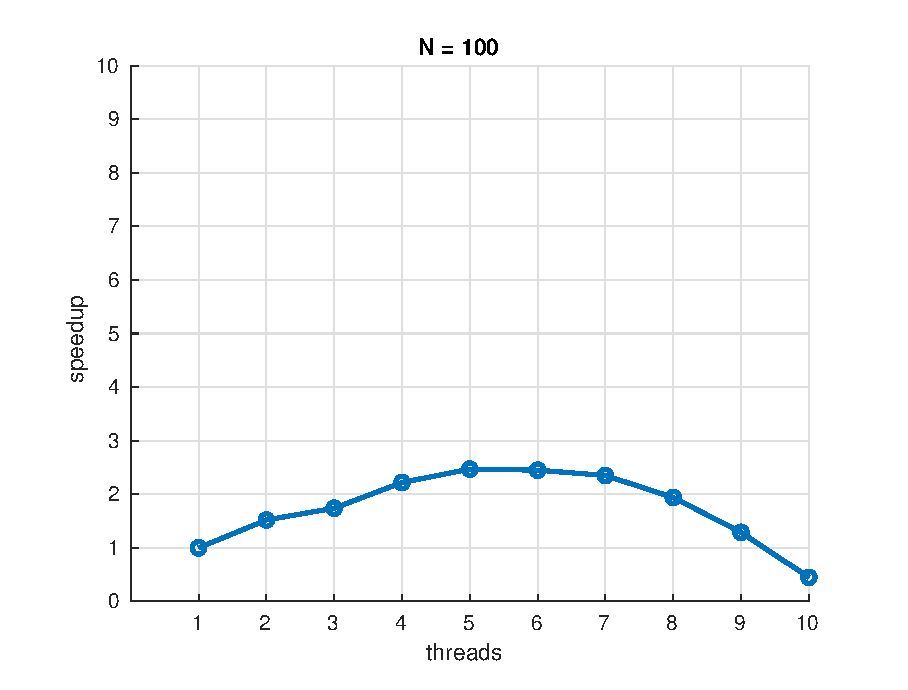
\includegraphics[width=3.2in]{fig/speedup100.eps}
\end{figure}

With an input size of 100 points, the speedup is very low due to the thread management overhead. With this relatively small input size it is not convenient to use a multithreading version of the algorithm.

\begin{table}[H]
\begin{tabular}{c c c}
\hline
\textbf{Number of points} & \multicolumn{2}{l}{1000} \\
\hline
\textbf{Sequential time} & \multicolumn{2}{l}{0.6094} \\
\hline
\textbf{Threads} & \textbf{Time} (seconds) & \textbf{Speedup} \\
\hline
2 & 0.2983 & 2.04 \\
3 & 0.1998 & 3.05 \\
4 & 0.1512 & 4.03 \\
5 & 0.1424 & 4.28 \\
6 & 0.1170 & 5.21 \\
7 & 0.1073 & 5.68 \\
8 & 0.0992 & 6.14 \\
9 & 0.1015 & 6.00 \\
10 & 0.0955 & 6.37 \\
\end{tabular}
\end{table}

\begin{figure}[H]
\centering
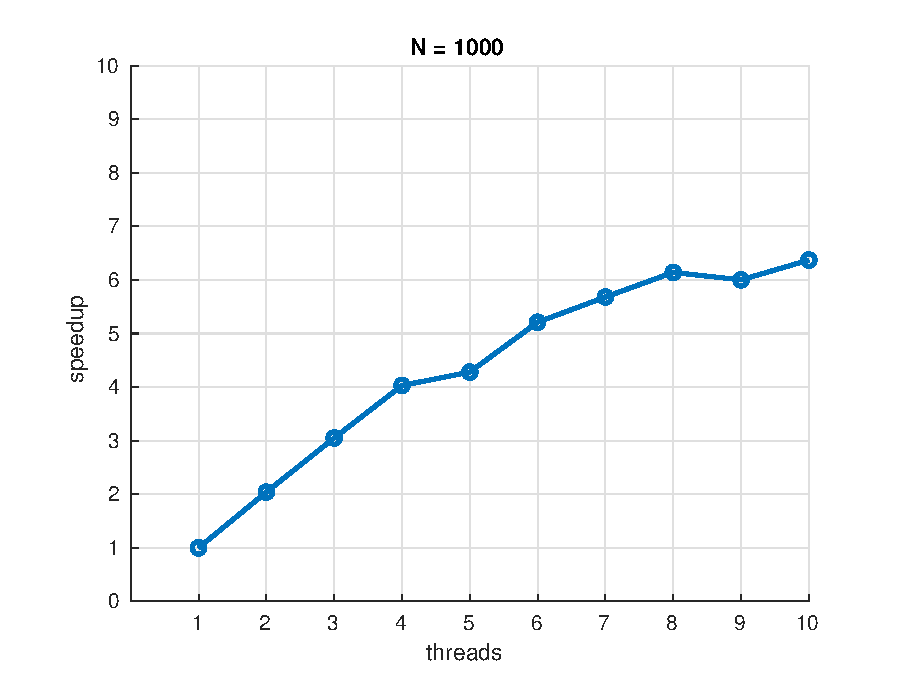
\includegraphics[width=3.2in]{fig/speedup1000.eps}
\end{figure}

Running the algorithm with an input size of 1000 make the parallel version run faster. The input size is large enough to get improvements by using a multithread version.

\begin{table}[H]
\centering
\begin{tabular}{ccc}
\hline
\textbf{Number of points} & \multicolumn{2}{l}{10000} \\
\hline
\textbf{Sequential time} & \multicolumn{2}{l}{54.1719} \\
\hline
\textbf{Threads} & \textbf{Time} (seconds) & \textbf{Speedup} \\
\hline
2 & 27.42 & 1.98 \\
3 & 18.36 & 2.95 \\
4 & 13.72 & 3.95 \\
5 & 12.44 & 4.35 \\
6 & 12.25 & 4.42 \\
7 & 10.83 & 5.00 \\
8 & 10.11 & 5.36 \\
9 & 10.50 & 5.16 \\
10 & 10.42 & 5.20 \\
\hline
\end{tabular}
\end{table}

\begin{figure}[H]
\centering
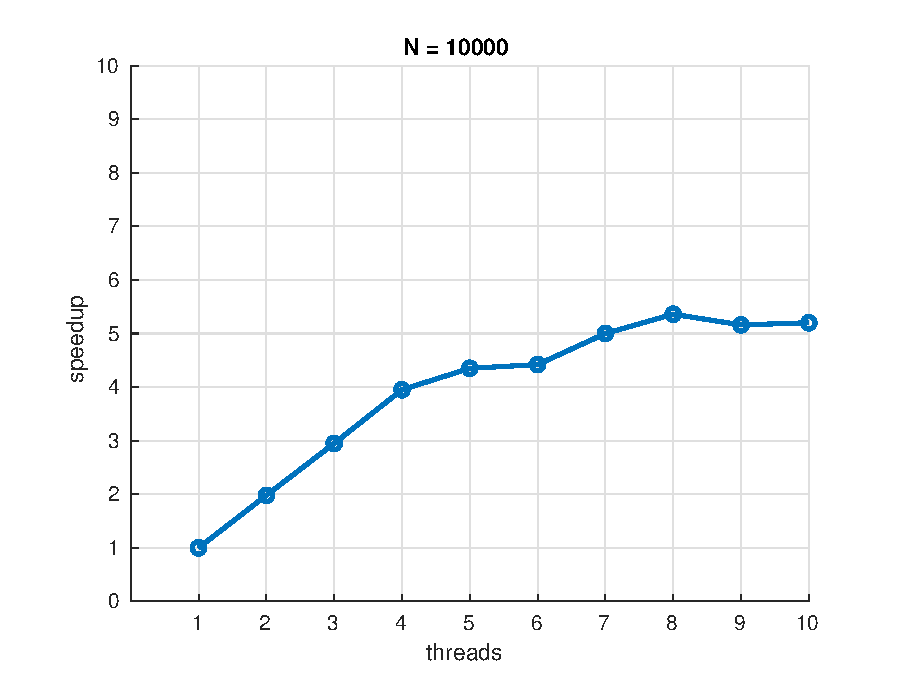
\includegraphics[width=3.2in]{fig/speedup10000.eps}
\end{figure}

\begin{table}[H]
\centering
\begin{tabular}{ccc}
\hline
\textbf{Number of points} & \multicolumn{2}{l}{20000} \\
\hline
\textbf{Sequential time} & \multicolumn{2}{l}{228.45} \\
\hline
\textbf{Threads} & \textbf{Time} (seconds) & \textbf{Speedup} \\
\hline
2 & 115.01 & 1.98 \\
3 & 76.06 & 3.00 \\
4 & 57.09 & 4.00 \\
5 & 52.99 & 4.31 \\
6 & 50.14 & 4.55 \\
7 & 47.09 & 4.58 \\
8 & 44.46 & 5.13 \\
9 & 45.09 & 5.07 \\
10 & 44.88 & 5.09 \\
\hline
\end{tabular}
\end{table}

\begin{figure}[H]
\centering
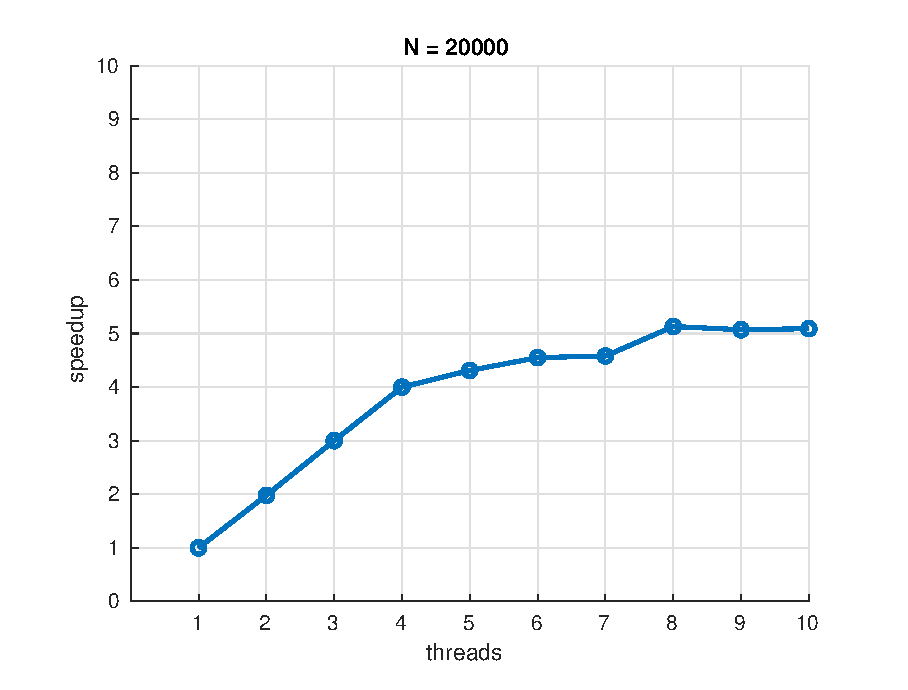
\includegraphics[width=3.2in]{fig/speedup20000.eps}
\end{figure}

\begin{table}[H]
\centering
\begin{tabular}{ccc}
\hline
\textbf{Number of points} & \multicolumn{2}{l}{50000} \\
\hline
\textbf{Sequential time} & \multicolumn{2}{l}{1398.49 \textit{s}} \\
\hline
\textbf{Threads} & \textbf{Time} (seconds) & \textbf{Speedup} \\
\hline
2 & 695.05 & 2.01 \\
3 & 465.51 & 3.00 \\
4 & 345.51 & 4.05 \\
5 & 325.10 & 4.30 \\
6 & 306.65 & 4.56 \\
7 & 289.90 & 4.82 \\
8 & 277.06 & 5.05 \\
9 & 274.78 & 5.09 \\
10 & 274.82 & 5.09 \\
\hline
\end{tabular}
\end{table}

\begin{figure}[H]
\centering
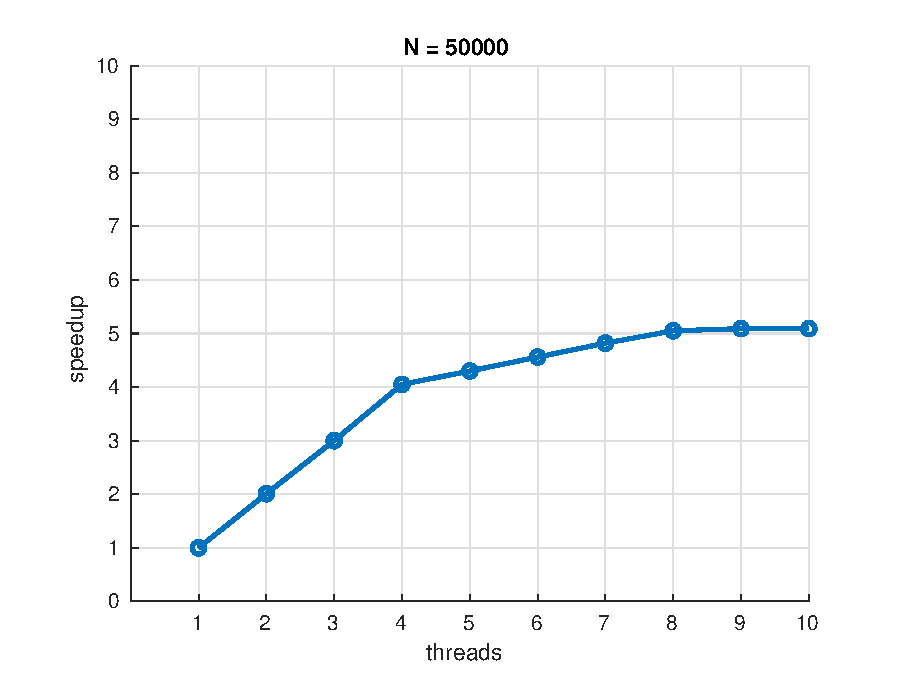
\includegraphics[width=3.2in]{fig/speedup50000.eps}

\end{figure}
The speedup seems to grow with three different patterns. From two threads to four threads the speeup is almost perfectly linear, from five to eight it seems to be sub-linear and over eight threads it stops growing.

\begin{figure}[H]
\centering
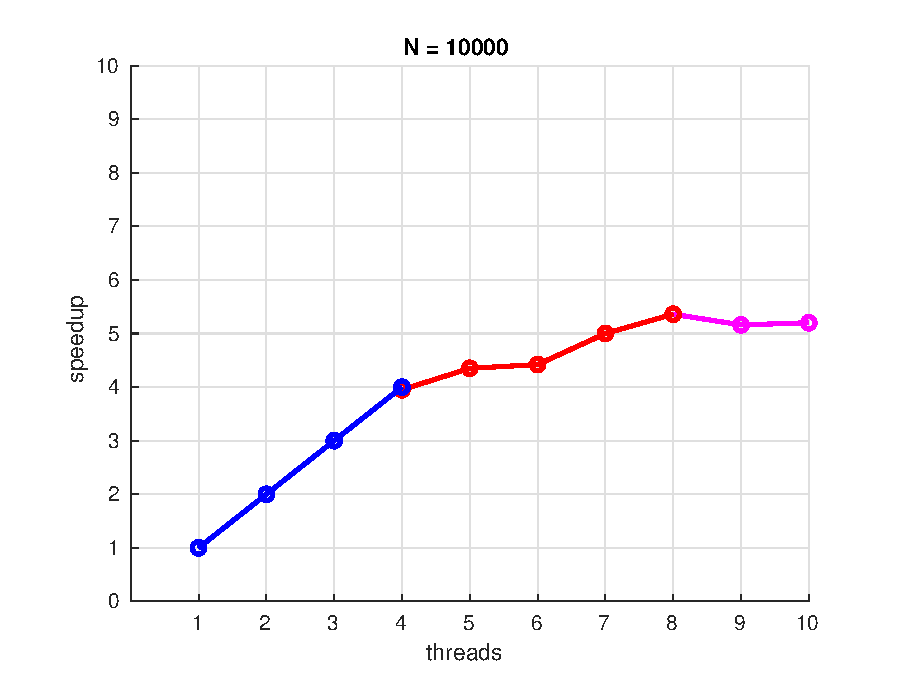
\includegraphics[width=3.2in]{fig/speedup10000Colors.eps}
\end{figure}

The explanation for these three different growing trends is immediate. The machine where the test was performed has the hyperthreading technology enabled: it shows eight cores but actually it has only four physical cores, the other four cores are virtual. In fact, from two to four threads the speedup is linear because each physical core has to execute a single thread. Using from five to eight threads can speed up the execution, but the speedup is no more perfectly linear, because there are more threads than physical cores. Finally over eight threads there is no more improvements in terms of speeds, on the contrary, it is slightly slower due to the overhead of the contex switches between threads.

In all the previous benchmarks the bandwith parameter is set at 3. Here are reported some benchmarks results where the input size is fixed at 10000 and the bandwith parameter equals to 1, 2 and 10.

\begin{table}[H]
\centering
\begin{tabular}{ccc}
\hline
\textbf{Bandwith} & \multicolumn{2}{l}{1} \\
\hline
\textbf{Sequential time} & \multicolumn{2}{l}{10.082 \textit{s}} \\
\hline
\textbf{Threads} & \textbf{Time} (seconds) & \textbf{Speedup} \\
\hline
2 & 5.30  & 1.90 \\
3 & 3.54 & 2.84 \\
4 & 2.83 & 3.565 \\
5 & 2.23 & 4.52 \\
6 & 1.91 & 5.27 \\
7 & 1.90 & 5.31 \\
8 & 2.03 & 4.97 \\
9 & 1.92 & 5.24 \\
10 & 1.95 & 5.18 \\
\hline
\end{tabular}
\end{table}

\begin{figure}[H]
\centering
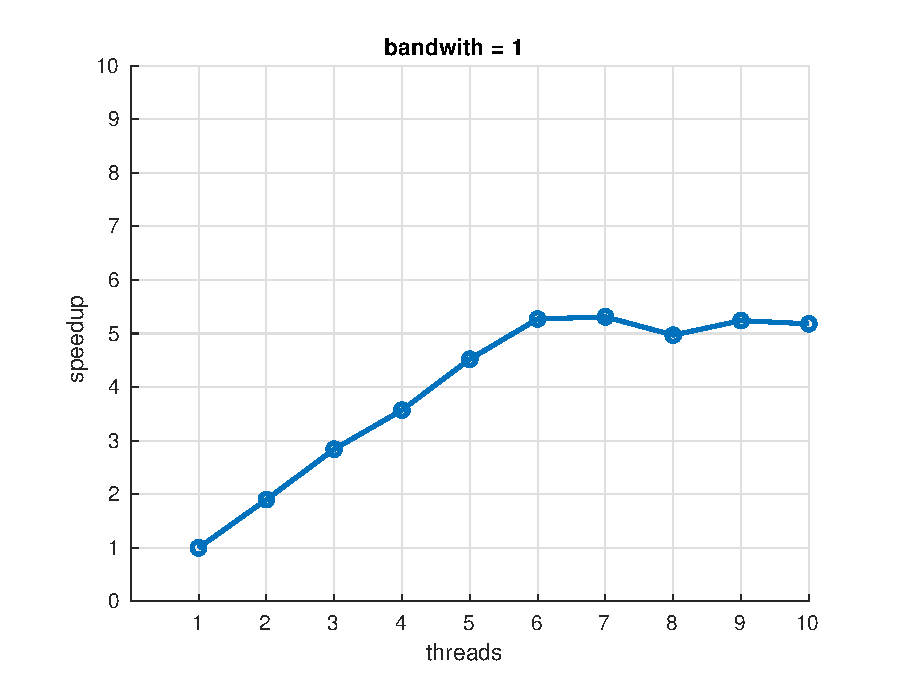
\includegraphics[width=3.2in]{fig/speedup1b.eps}
\end{figure}

\begin{table}[H]
\centering
\begin{tabular}{ccc}
\hline
\textbf{Bandwith} & \multicolumn{2}{l}{2} \\
\hline
\textbf{Sequential time} & \multicolumn{2}{l}{9.082 \textit{s}} \\
\hline
\textbf{Threads} & \textbf{Time} (seconds) & \textbf{Speedup} \\
\hline
2 & 4.86  & 1.91 \\
3 & 3.27 & 2.83 \\
4 & 2.45 & 3.78 \\
5 & 1.96 & 4.72 \\
6 & 1.96 & 4.74 \\
7 & 1.65 & 5.61 \\
8 & 1.59 & 5.81 \\
9 & 1.62 & 5.71 \\
10 & 1.80 & 5.16 \\
\hline
\end{tabular}
\end{table}

\begin{figure}[H]
\centering
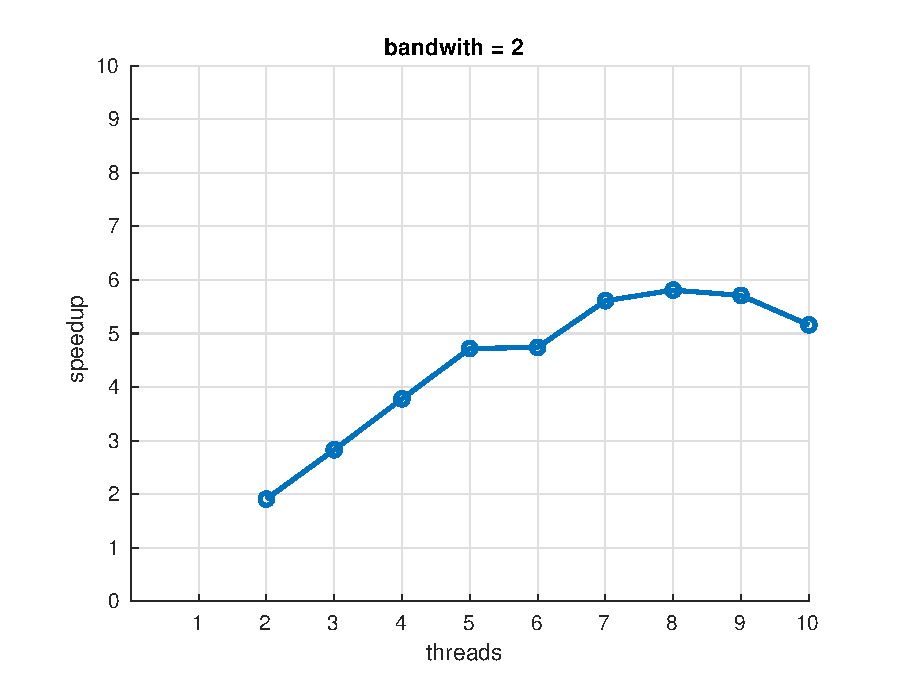
\includegraphics[width=3.2in]{fig/speedup2b.eps}
\end{figure}

\begin{table}[H]
\centering
\begin{tabular}{ccc}
\hline
\textbf{Bandwith} & \multicolumn{2}{l}{10} \\
\hline
\textbf{Sequential time} & \multicolumn{2}{l}{52.11 \textit{s}} \\
\hline
\textbf{Threads} & \textbf{Time} (seconds) & \textbf{Speedup} \\
\hline
2 & 26.27 & 1.98 \\
3 & 17.58 & 2.96 \\
4 & 13.41 & 3.88 \\
5 & 12.14 & 4.29 \\
6 & 11.67 & 4.47 \\
7 & 10.73 & 4.85 \\
8 & 10.16 & 5.13 \\
9 & 10.22 & 5.10 \\
10 & 10.07 & 5.18 \\
\hline
\end{tabular}
\end{table}

\begin{figure}[H]
\centering
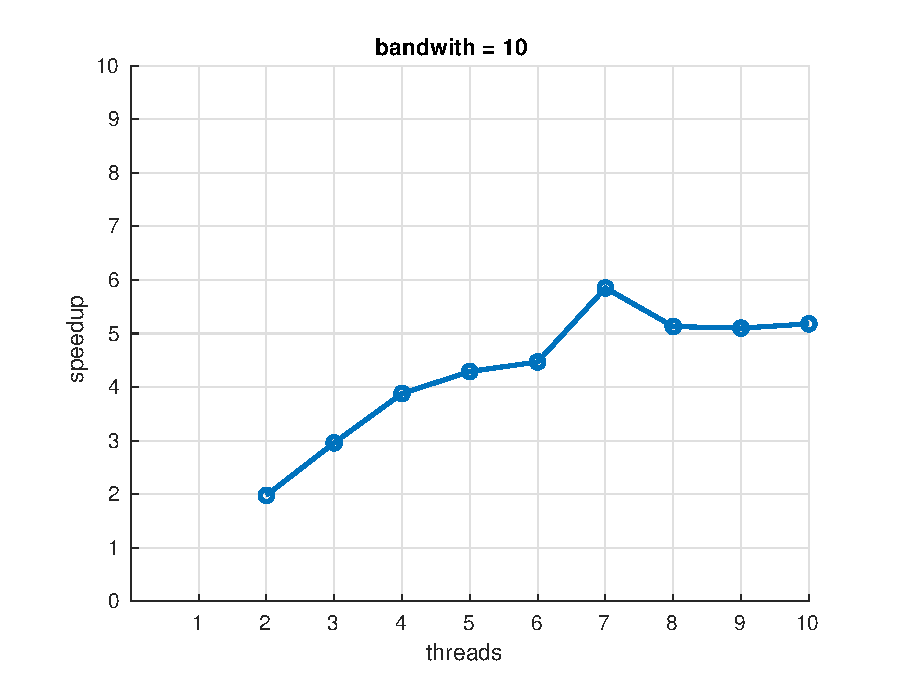
\includegraphics[width=3.2in]{fig/speedup10b.eps}
\end{figure}

The growing trends from one to four cores seem to be almost all the same for every value of the bandwith parameter. So we can conclude that if the dataset is big enough, the choice of the bandwith parameter will not influence the speedup.

\end{document}
